\documentclass[10pt]{beamer}
\usetheme{pohan}
\usepackage{lipsum}
\usepackage{tabularx}
\usepackage{xcolor}
\usepackage{fancybox, graphicx}
\usepackage{animate}



\renewcommand{\arraystretch}{2}
\renewcommand\tabularxcolumn[1]{m{#1}}
\title{BERT}
\subtitle{\textcolor{Primary}{B}idirectional \textcolor{Primary}{E}ncoder \textcolor{Primary}{R}epresentations from \textcolor{Primary}{T}ransformer}
\author{Team 7}
\date{\today}


\begin{document}

\maketitle

\maketoc

\section{Transformer}

\begin{frame}{Transformer}
  
  \begin{figure}
    \centering
    \shadowbox{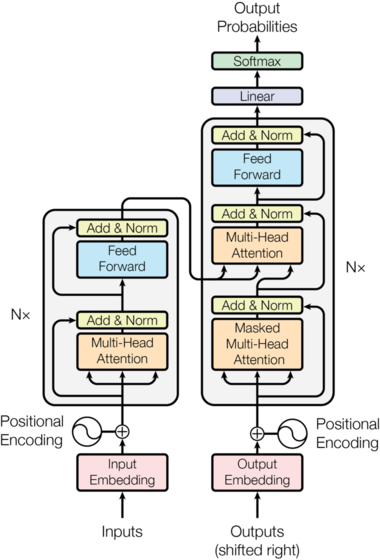
\includegraphics[height=0.7\textheight]{img_dir/transformer}}
    \caption{\textbf{Transformer}: Attention is all you need }
  \end{figure}

\end{frame}

  \begin{frame}{Overview}
    \begin{figure}
      \centering
      \shadowbox{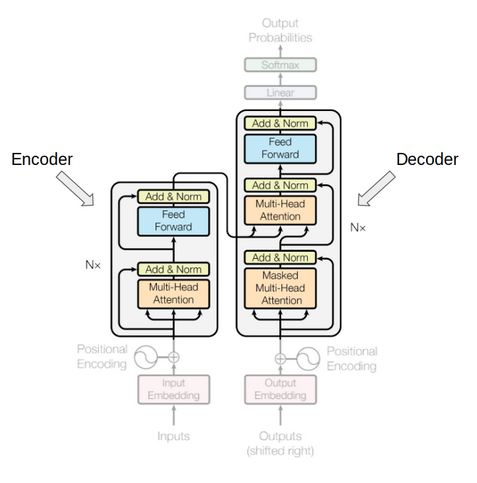
\includegraphics[height=0.7\textheight]{img_dir/Encoder-Decoder}}
      \caption{\textbf{Encoder-Decoder} }
    \end{figure}
  \end{frame}

  \subsection{Encoder}

  \begin{frame}{Encoder}
    \begin{figure}
      \centering
      \shadowbox{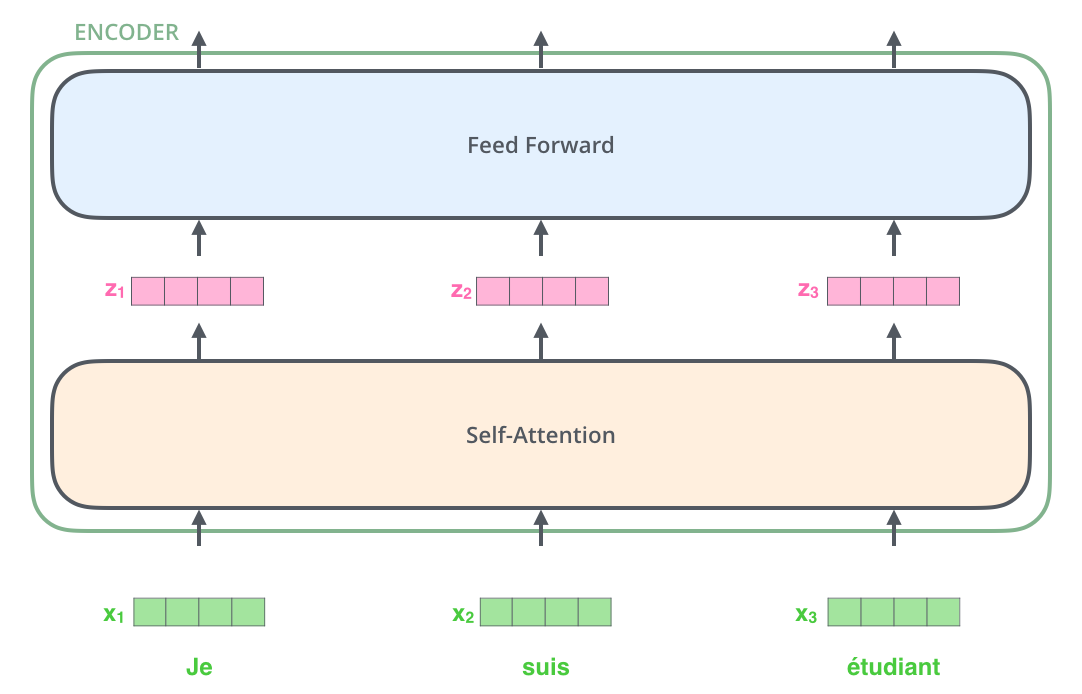
\includegraphics[height=0.7\textheight]{img_dir/encoder_with_tensors}}
      \caption{\textbf{1 Encoder-layer} }
      \label{fig:Encoder}
    \end{figure}
  \end{frame}

  \subsection{Self-Attention}

  \begin{frame}{Self-Attention}
    \begin{figure}
      \centering
      \shadowbox{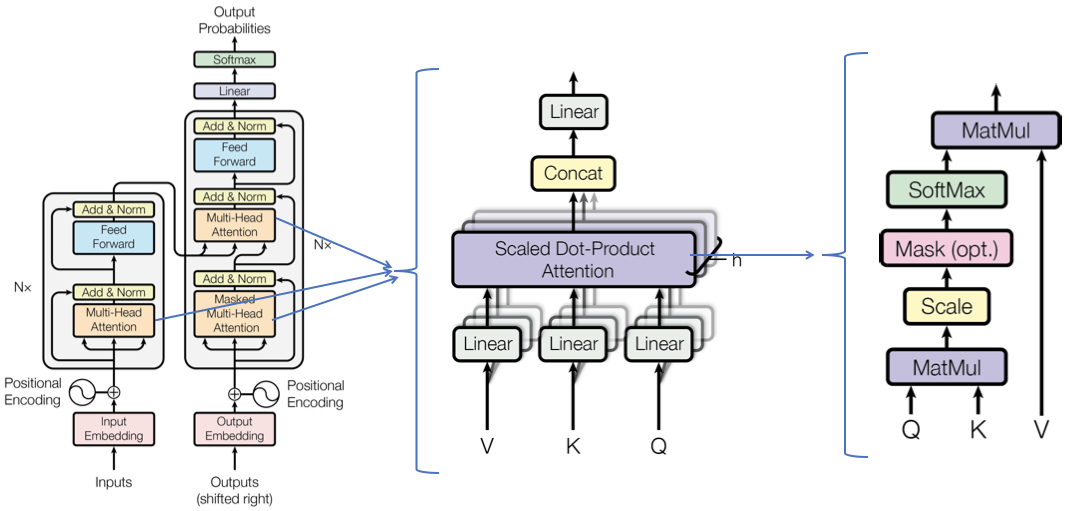
\includegraphics[width=0.9\textwidth]{img_dir/self-attention}}
      \caption{\textbf{Self-Attention} }
      \label{fig:Self-Attention}
    \end{figure}
  \end{frame}

\section{BERT}

  \begin{frame}{BERT}
    \begin{figure}
      \centering
      \shadowbox{
\includegraphics[width=0.5\textwidth]{img_dir/Bert}}
      \caption{\textbf{BERT} }
      \label{fig:BERT}
    \end{figure}
  \end{frame}

  \subsection{Archtecture \& Input}
  
  \begin{frame}{Archtecture}
    \begin{figure}
      \centering
      \shadowbox{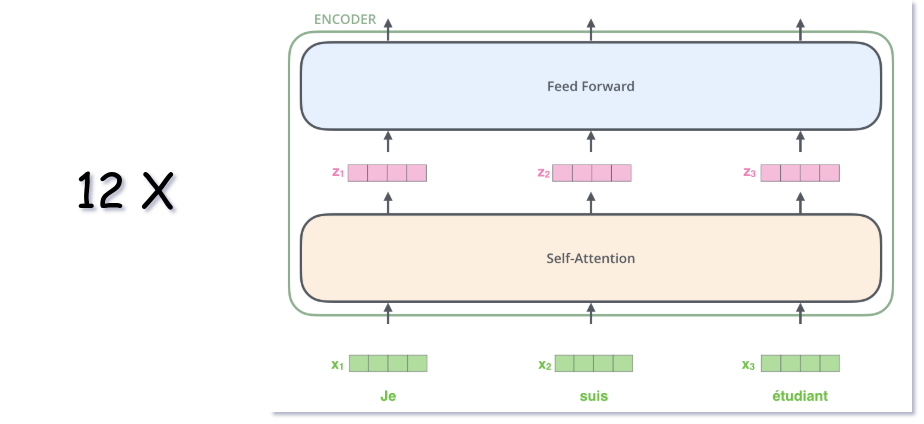
\includegraphics[width=0.7\textwidth]{img_dir/BERT-intuition} } 
      \caption{\textbf{BERT-Architecture} }
    \end{figure}
  \end{frame}

  \begin{frame}{Input}
    \begin{figure}
      \centering
      \shadowbox{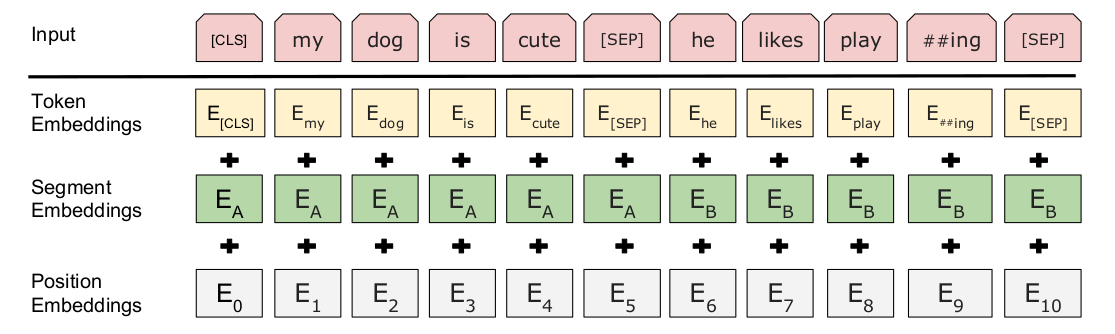
\includegraphics[width=0.9\textwidth]{img_dir/input} } 
      \caption{\textbf{BERT-Input} }
    \end{figure}
  \end{frame}

  \subsection{2 stage Training}

  \begin{frame}{2-stage-training}

    \begin{exampleblock}{Pre-training}
      Self-supervised tasks.
    \end{exampleblock}

      \begin{exampleblock}{Finetune}
        3 finetune tasks.
      \end{exampleblock}

  \end{frame}

  \subsection{Pre-Training}

  \begin{frame}{Pre-Training}

    \begin{exampleblock}{Pretraining tasks}
      2 pretraining tasks
    \end{exampleblock}

      \begin{exampleblock}{NSP}
        Next Sentence Prediction
      \end{exampleblock}

      \begin{exampleblock}{MLM}
        Masked Language Model - self supervised learning
      \end{exampleblock}
  \end{frame}

  \subsubsection*{Next Sentence Prediction}
  \begin{frame}{NSP}
    \begin{figure}
      \centering
      \shadowbox{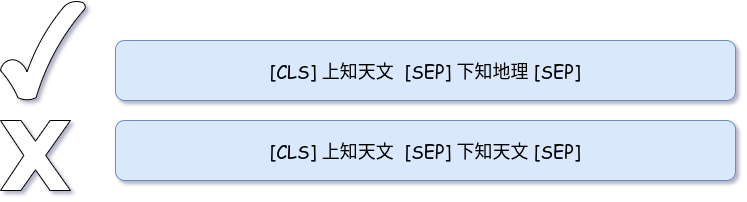
\includegraphics[width=0.9\textwidth]{img_dir/nsp} } 
      \caption{\textbf{Next Sentence Prediction} }
    \end{figure}
    \begin{figure}
      \centering
      \shadowbox{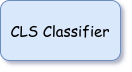
\includegraphics[width=0.25\textwidth]{img_dir/cls} } 
      \caption{\textbf{[CLS] token classifier} }
    \end{figure}
  \end{frame}

  \subsection{self-supervised learning}

  \begin{frame}{SSL}

    What is self-supervised learning ?
    \begin{figure}
      \centering
      \shadowbox{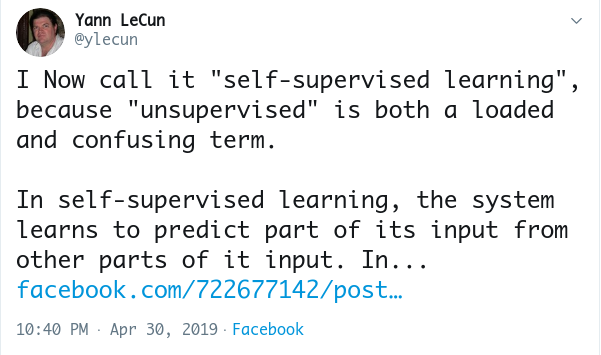
\includegraphics[width=0.7\textwidth]{img_dir/self-supervised} } 
      \caption{\textbf{Self-supervised learning definition} }
    \end{figure}

  \end{frame}

  \subsubsection*{Masked LM}
  \begin{frame}{MLM}
    \begin{figure}
      \centering
      \shadowbox{\includegraphics[width=0.7\textwidth]{img_dir/MASKLM} } 
      \caption{\textbf{Masked LM} }
    \end{figure}
    \begin{figure}
      \centering
      \shadowbox{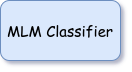
\includegraphics[width=0.25\textwidth]{img_dir/mlm} } 
      \caption{\textbf{MLM classifier} }
    \end{figure}
  \end{frame}

  \subsection{FineTune}

  \begin{frame}{Fine-Tune}
  Downstream tasks:
  \begin{exampleblock}{NER}
    Name Entity Recognition
  \end{exampleblock}

  \begin{exampleblock}{NLI}
    Natural Language Inference
  \end{exampleblock}

  \begin{exampleblock}{QA}
    Question Answering
  \end{exampleblock}

  \end{frame}

  \subsubsection*{NLI}

  \begin{frame}{NLI}
    \begin{figure}
      \centering
      \shadowbox{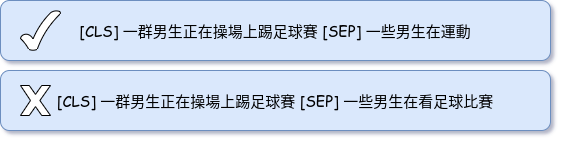
\includegraphics[width=0.9\textwidth]{img_dir/nli} } 
      \caption{\textbf{Natural Language Inference} }
    \end{figure}
    \begin{figure}
      \centering
      \shadowbox{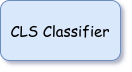
\includegraphics[width=0.25\textwidth]{img_dir/cls} } 
      \caption{\textbf{[CLS] token classifier} }
    \end{figure}
  \end{frame}

  \subsubsection*{QA}

  \begin{frame}{QA}
    \begin{figure}
      \centering
      \shadowbox{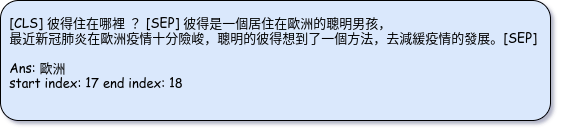
\includegraphics[width=0.9\textwidth]{img_dir/qa} } 
      \caption{\textbf{Question Answering Example} }
    \end{figure}
    \begin{figure}
      \centering
      \shadowbox{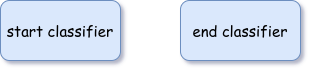
\includegraphics[width=0.6\textwidth]{img_dir/start_end} } 
      \caption{\textbf{Random initialize two classifiers} }
    \end{figure}

  \end{frame}

  \subsection{Conclusion}

  \begin{frame}{Conclusion}
    2-stage training
    \begin{figure}
      \centering
      \shadowbox{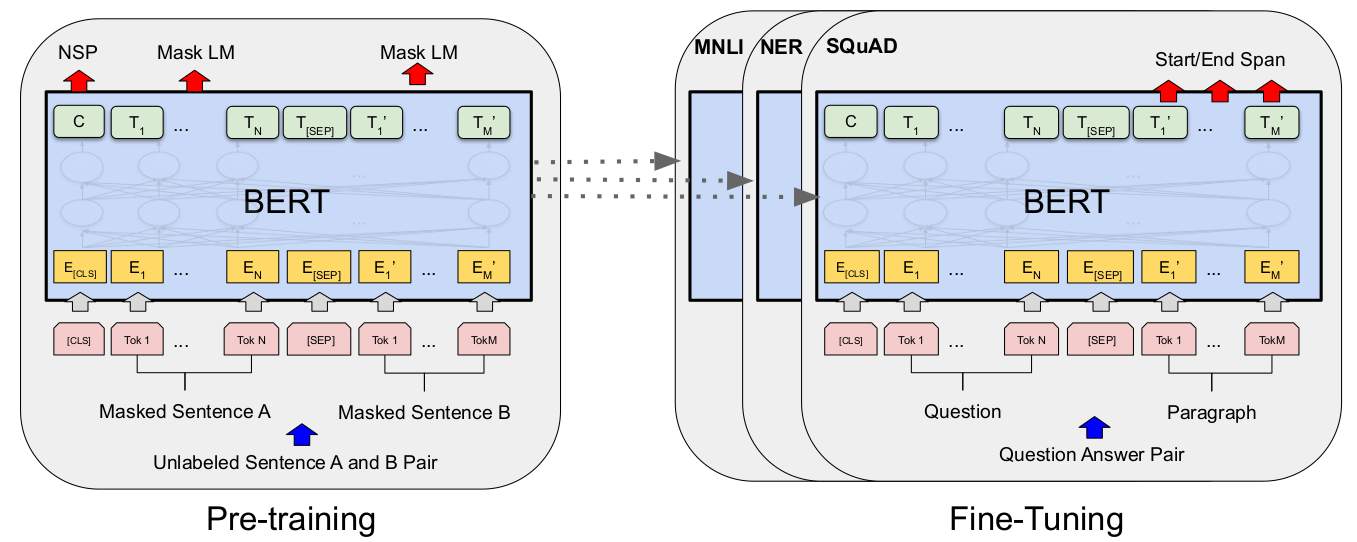
\includegraphics[width=0.95\textwidth]{img_dir/pretrain-finetine} } 
      \caption{\textbf{2-stage training} }
    \end{figure}
  \end{frame}

\section{BERT-Family}

  \begin{frame}{BERT-Family (1)}
    \begin{figure}
      \centering
      \shadowbox{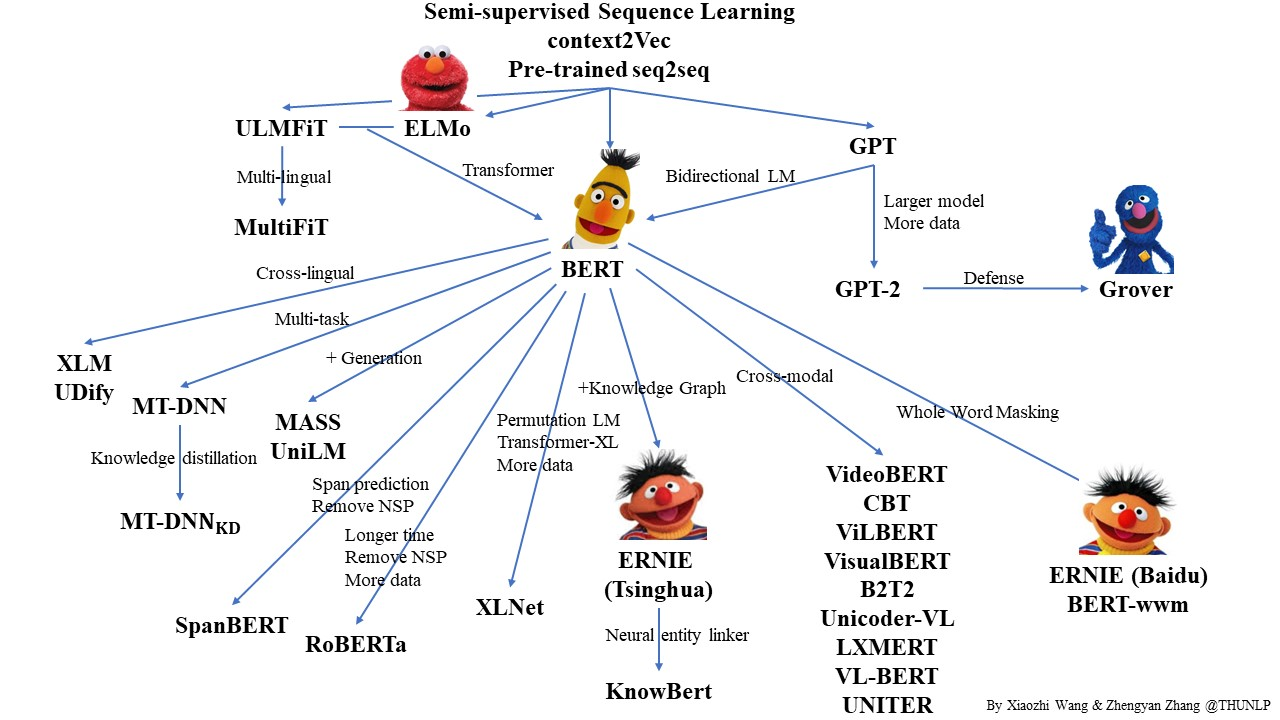
\includegraphics[width=0.95\textwidth]{img_dir/PLMfamily} } 
      \caption{\textbf{BERT Family} }
    \end{figure}
  \end{frame}

  \begin{frame}{BERT-Family (2)}

    \begin{exampleblock}{SpanBERT - EMNLP2019}
      Improving Pre-training by Representing and Predicting Spans
    \end{exampleblock}

    \begin{exampleblock}{Roberta - ICLR2020 Reject}
      A Robustly Optimized BERT Pretraining Approach
    \end{exampleblock}

    \begin{exampleblock}{ALBERT - ICLR2020 Spotlight}
      A Lite BERT for Self-supervised Learning of Language Representations
    \end{exampleblock}
  
  \end{frame}

  \subsection{SpanBERT, Roberta, ALBERT}

    \begin{frame}{SpanBERT, Roberta, ALBERT}
      \begin{exampleblock}{Difference with BERT    - SpanBERT}
        1. change NSP task to SBO (span boundary objective) task.

        2. mask random consecutive spans.   

      \end{exampleblock}

      \begin{exampleblock}{Difference with BERT    - Roberta}

        1. More big batch size when training bert.
 
        2. More optimal hyperparameters.
 
        3. More data.

        4. Remove NSP task.
       \end{exampleblock}

       \begin{exampleblock}{Difference with BERT   - ALBERT}

        1. change NSP task to SOP (Sentence Order Prediction) task.

        2. One layer recall 12 times to build 12 layers. (share parameters)
 
        3. factorize embedding table. initize small and project to big dimension.
       \end{exampleblock}


    \end{frame}

\end{document}
